\chapter{Interfaz}
\label{cap:interfaz}

En cuanto a la interfaz de la página web, uno de los principales objetivos del presente trabajo era aunar todas las funcionalidades de la aplicación original, así como las extensiones implementadas en este desarrollo, en una única interfaz web, mediante la cual el usuario pueda navegar y acceder a todas las funcionalidades disponibles.

El resultado de este objetivo está recogido en este capítulo. Para alcanzarlo, se han creado vistas completamente nuevas y se han modificado algunas de las vistas previamente existentes para simplificarlas o añadir funcionalidades.

\section{Proceso de diseño de la interfaz}

Para desarrollar estas vistas, se ha tenido en cuenta y dado un peso importante al desarrollo empleando el diseño centrado en el usuario, empleando los métodos de colaboración con potenciales clientes de la aplicación, análisis de otras herramientas similares y adaptando el diseño dependiendo del tamaño del dispositivo, como se explica en una de las guías sobre diseño centrado en el usuario \citep{pratt2012interactive}. El siguiente paso a tomar, según esta guía, es el de experimentación y validación con los usuarios finales, el cual se realizará una vez la aplicación esté en funcionamiento, pudiendo así adaptar los \textit{workflows}, botones o maquetación a un entorno más adaptado a los usuarios.

Dentro de este ámbito de diseño centrado en el usuario, y como también se mencionó en el capítulo 2 (el Estado de la Cuestión), se ha tenido especial atención a la democratización del uso de esta aplicación, por lo que uno de los objetivos principales con el diseño era implementar una interfaz sencilla, usable e intuitiva para que cualquier usuario pudiera utilizarla fácilmente.

Para demostrar el uso del diseño centrado en el usuario a lo largo de este proyecto, a continuación expondremos un ejemplo en el que se siguen los pasos claros de comprensión de la experiencia de usuario, especificación de las necesidades del usuario, diseño de la solución y evaluación de la misma en el ejemplo concreto del diseño de una simulación disponible en la vista de 'Visualizar Simulaciones', del cual se pueden ver capturas más abajo, en la correspondiente sección \ref{vistaVisSim}, que trata sobre esta vista.

\begin{itemize}
	
	\item \textbf{Comprensión}: El primer paso para diseñar este apartado, al igual que todos los elementos de nuestra interfaz, fue el de la comprensión de cómo el usuario experimentará con el producto. Visto desde un punto de vista más general, dentro de la página de 'Visualizar simulaciones' habría una lista que contendría las simulaciones, el contenido en estas tarjetas debía ser limitado pero suficientemente explicativo para que el usuario lo comprendiese.
	
	\item \textbf{Especificación}: Una vez investigamos y comprendimos el flujo de experiencia de usuario para este elemento, y cómo se relaciona con  los demás elementos, se especifican los requerimientos de lo que esperaría ver un usuario si interactuase con este elemento. Como ya mencionamos, es importante que esta información sea breve pero explicativa.
		
	Por tanto, se decidió que este elemento contuviese la información básica para distinguir la simulación entre otras. Incluimos en este elemento información sobre el mapa, la simulación sobre la que está realizada, step en el que se desea comenzar la visualización, velocidad de reproducción, botón de inicio y resto de metainformación (como puede ser fecha y hora de inicio o resumen de la simulación).
	
	\item \textbf{Diseño}: Una vez comprendido el contexto y requerimientos de los usuarios, se pasa a la fase de diseño de la solución en sí. Como ya se conocía el contenido que debía tener, es necesario dividir la información en el reducido espacio de la tarjeta para que resulte atractivo y sencillo.
	
	La decisión que tomamos respecto a esto es indicar el mapa en la sección izquierda, el título en grande, diferenciando cada simulación y acompañado de un enlace a la simulación padre en pequeño. Después, habría dos inputs donde indicar el step y velocidad, junto con el botón de inicio. Por último, se ndicaría toda la metainformación y, si esta ocupase múltiples líneas, se permitiría el 'scroll' dentro de la tarjeta, para que no ocupe demasiado espacio vertical.
	
	\item \textbf{Evaluación}: Finalmente, una vez hemos construido el elemento, con la información especificada y el diseño pertinente, es necesario ratificar todo el conjunto para comprobar la validez. Esto se puede hacer mediante pruebar realizadas por nosotros mismos en etapas de desarrollo, mediante pruebas de conocidos, utilizando la aplicación por su cuenta e informando de los resultados, o con el producto final funcionando, recibiendo feedback de los usuarios reales y adaptando todo el proceso de diseño, cambiando lo necesario en cada paso.
	
\end{itemize}

Estos cuatro pasos de diseño forman parte de del proceso de diesño que explica Google en su curso de diseño de UX profesional \footnote{\url{https://www.coursera.org/google-certificates/certificado-diseno-de-experiencia-del-usuario-ux}}, y se ven indicados en la figura \ref{fig:pasosDisenoUsuario}.

\begin{figure}[H]
	\centering
	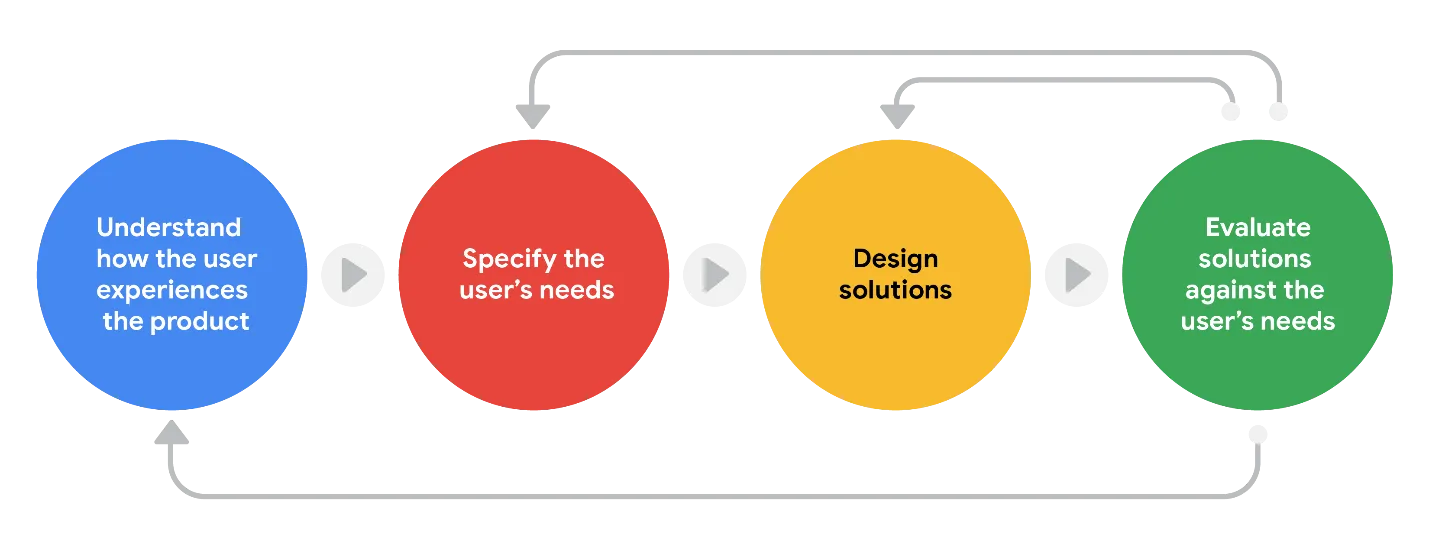
\includegraphics[width = 1\textwidth]{Imagenes/Vectorial/pasos_DCU.png}
	\caption{Pasos para diseño centrado en el usuario según Google}
	\label{fig:pasosDisenoUsuario}
\end{figure}

\section{Nuevas vistas}

En esta sección se presentan las vistas creadas durante el desarrollo del trabajo, las cuales sirven de apoyo para ejecutar las funcionalidades, tanto nuevas como existentes, de la aplicación.

Estas vistas no existían previamente en la aplicación, y se ha realizado un proceso de ingeniería inversa de las vistas preexistentes para poder adaptar las interfaces y que se comuniquen de manera efectiva con el back end.

Primeramente, atendiendo a la movilidad entre páginas, se ha implementado una barra de navegación, la cual compartirán todas las páginas y permitirá navegar entre las diferentes funcionalidades, como se puede apreciar en las figuras \ref{fig:navBarDesktop}, \ref{fig:navBarMobile1} y \ref{fig:navBarMobile2}.

\begin{figure}[H]
	\centering
	
\includegraphics[width = 1\textwidth]{Imagenes/Vectorial/navBarDesktop.png}
	\caption{Barra de navegación en el formato Desktop}
	\label{fig:navBarDesktop}
\end{figure}

\begin{figure}[H]
	\centering
	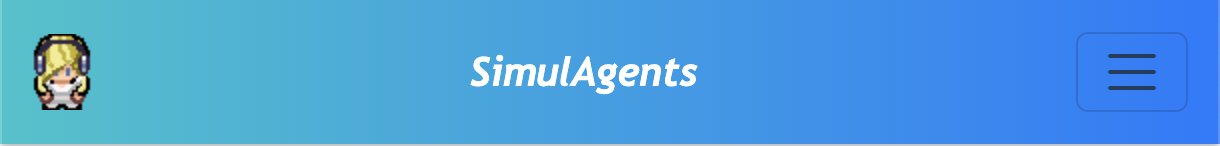
\includegraphics[width = 1\textwidth]{Imagenes/Vectorial/navBarMobile1.png}
	\caption{Barra de navegación en el formato para dispositivos móviles}
	\label{fig:navBarMobile1}
\end{figure}

\begin{figure}[H]
	\centering
	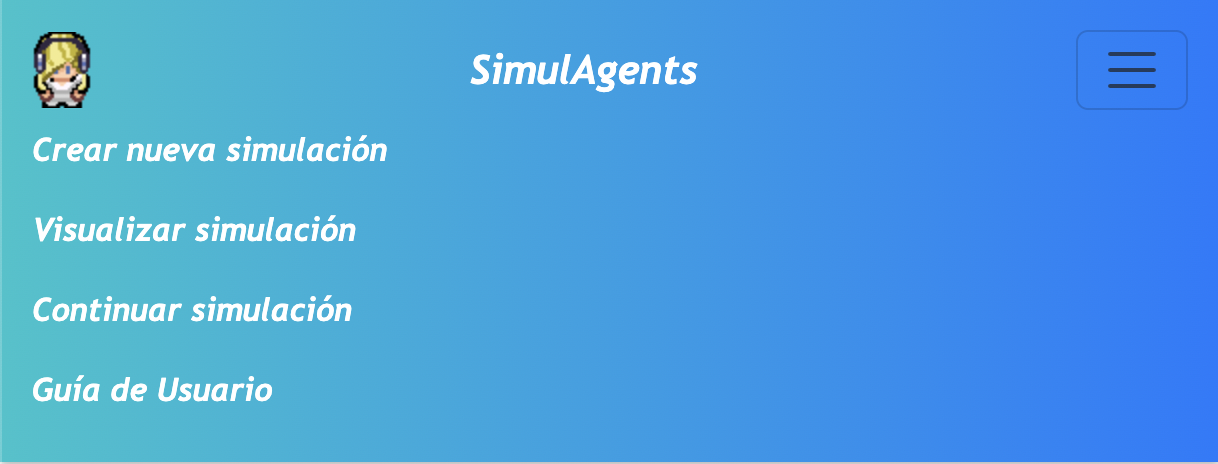
\includegraphics[width = 1\textwidth]{Imagenes/Vectorial/navBarMobile2.png}
	\caption{Barra de navegación en el formato para dispositivos móviles, con la barra de navegación desplegada}
	\label{fig:navBarMobile2}
\end{figure}

\subsection{Vista de Crear nueva simulación}

Teniendo en cuenta los objetivos y las funcionalidades implementadas en este trabajo, es evidente la necesidad de un apartado en el que permitir a los usuarios crear sus propias simulaciones. En esta vista, los usuarios primeramente indicarán el número de personajes que quieren que intervengan en la simulación.

Dependiendo del número de personajes deseados, mediante el uso de la tecnología JQuery, se mostrarán u ocultarán las casillas de relleno de la información de los personajes. Para cada uno de los agentes, los usuarios indicarán el nombre que le quieren dar y la personalidad de los mismos. Como se puede ver en la figura \ref{fig:vistaCrearSimulacion}, el apartado de personalidad viene separado por los siguientes conceptos:

\begin{itemize}
	
	\item \textbf{Personalidad innata}: El usuario escogerá entre un grupo de personalidades innatas preestablecidas, las cuales darán cierta profundidad a los personajes y constan de una sola palabra, que define simplemente el carácter de cada personaje.
	
	\item \textbf{Estilo de vida}: Aquí se explicará sobre cómo es el estilo de vida en general del personaje. Se dará una mayor profundidad al carácter, explicando sus hábitos, costumbres, vicios y virtudes.
	
	\item \textbf{Conocimiento aprendido}: Consistirá en una recopilación de todas las vivencias recopiladas por el personaje que puedan afectar a sus decisiones o su personalidad. Aquí se indicará, por ejemplo, qué tipo de relación tiene con el resto de personajes, si le caen bien o mal, qué experiencias tiene con ellos y demás información relevante para la simulación.
	
	\item \textbf{Estado actual}: Finalmente, se indicará la acción que está realizando en el momento de comienzo de la simulación, así como sus preocupaciones más inmediatas y las acciones que tomará en los próximos steps.
	
\end{itemize}

Con esta información, se podrá inferir la personalidad completa de cada uno de los personajes para así adaptarlos óptimamente a las simulaciones y tener una mayor granularidad al comparar las diferentes simulaciones, cambiando cierta parte de esta información y viendo cómo cambian los comportamientos

Si se quisiera aportar un contexto general a toda la simulación, la solución sería indicarlo en los apartados de conocimiento aprendido y estado actual de todos los personajes. Si todos ellos tienen una pieza de conocimiento aprendido común, podrán inferir la situación en la que se encuentran e interactuar con los demás porque también estarán en la misma situación.

Todos estos elementos gráficos se pueden apreciar en las figuras \ref{fig:vistaCrearSimulacion} y \ref{fig:vistaCrearSimulacionMobile}, donde se ve que el diseño es 'responsive' y se adapta a todo tipo de pantallas.

\begin{figure}[H]
	\centering
	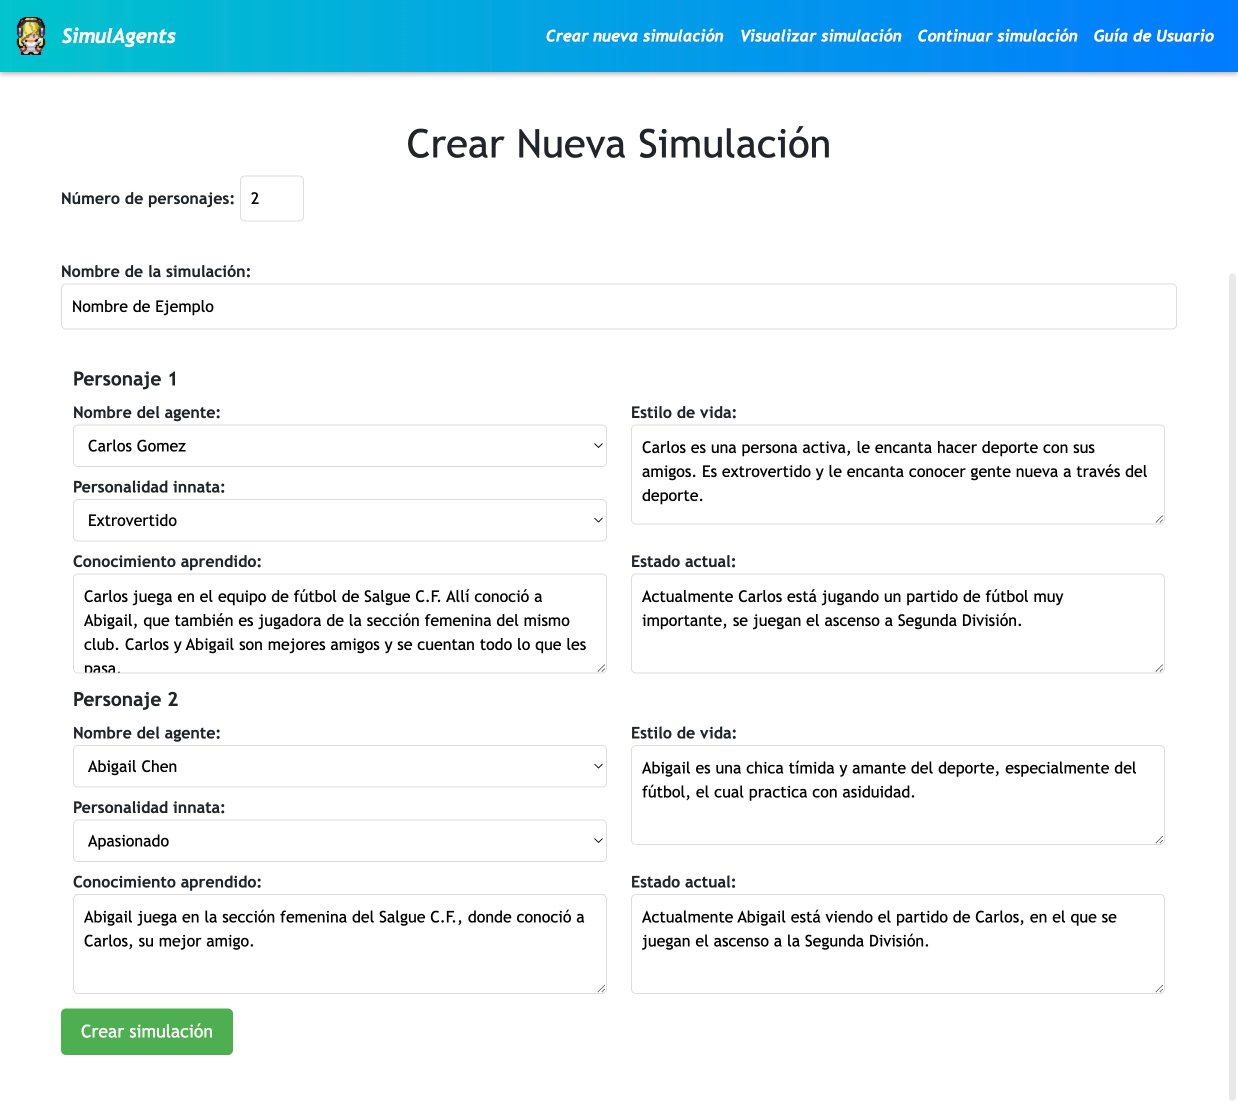
\includegraphics[width = 1\textwidth]{Imagenes/Vectorial/crearSimu.png}
	\caption{Versión de escritorio de la vista para crear una nueva simulación}
	\label{fig:vistaCrearSimulacion}
\end{figure}

\begin{figure}[H]
	\centering
	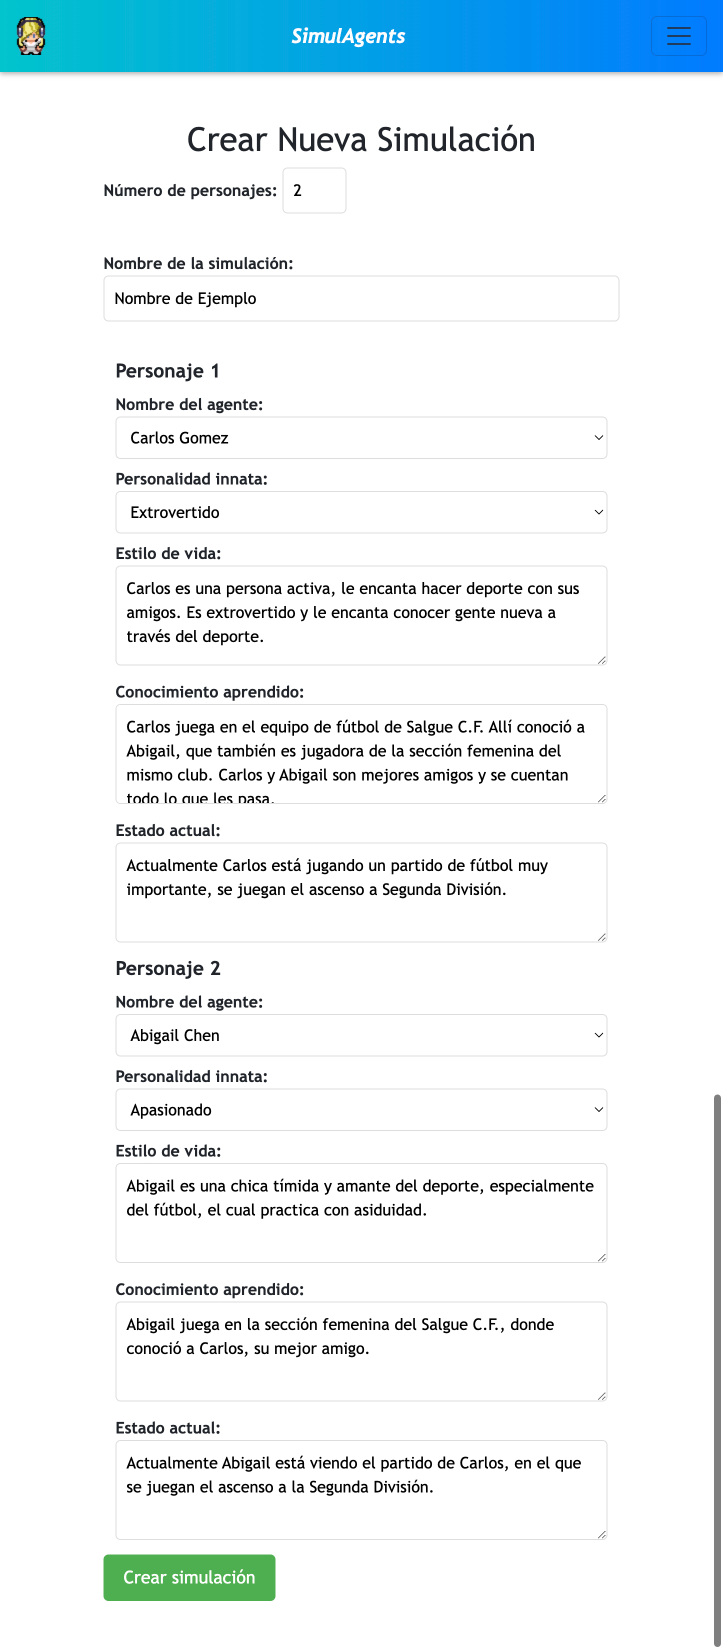
\includegraphics[width = 0.7\textwidth]{Imagenes/Vectorial/crearSimuMobile.png}
	\caption{Versión de móvil de la vista para crear una nueva simulación}
	\label{fig:vistaCrearSimulacionMobile}
\end{figure}

\subsection{Vista de Visualizar simulaciones}
\label{vistaVisSim}

En esta vista es donde los usuarios pueden seleccionar las simulaciones a visualizar. Esto es, las que se han ejecutado y guardado para visualizarlas previamente. Una vez se selecciona una de estas vistas, se accede a la interfaz de visualización de una simulación, la cual está explicada en profundidad en la subsección  \ref{sec:vistaSimulacion}.

Como ejemplo, se proporciona la figura \ref{fig:visSimDesktop} indicando cómo aparece esta vista representada en la página web. En este caso, también existe un diseño adaptado a dispositivos móviles, pero al ser similar a la versión de escritorio, se omite por simplicidad.

\begin{figure}[H]
	\centering
	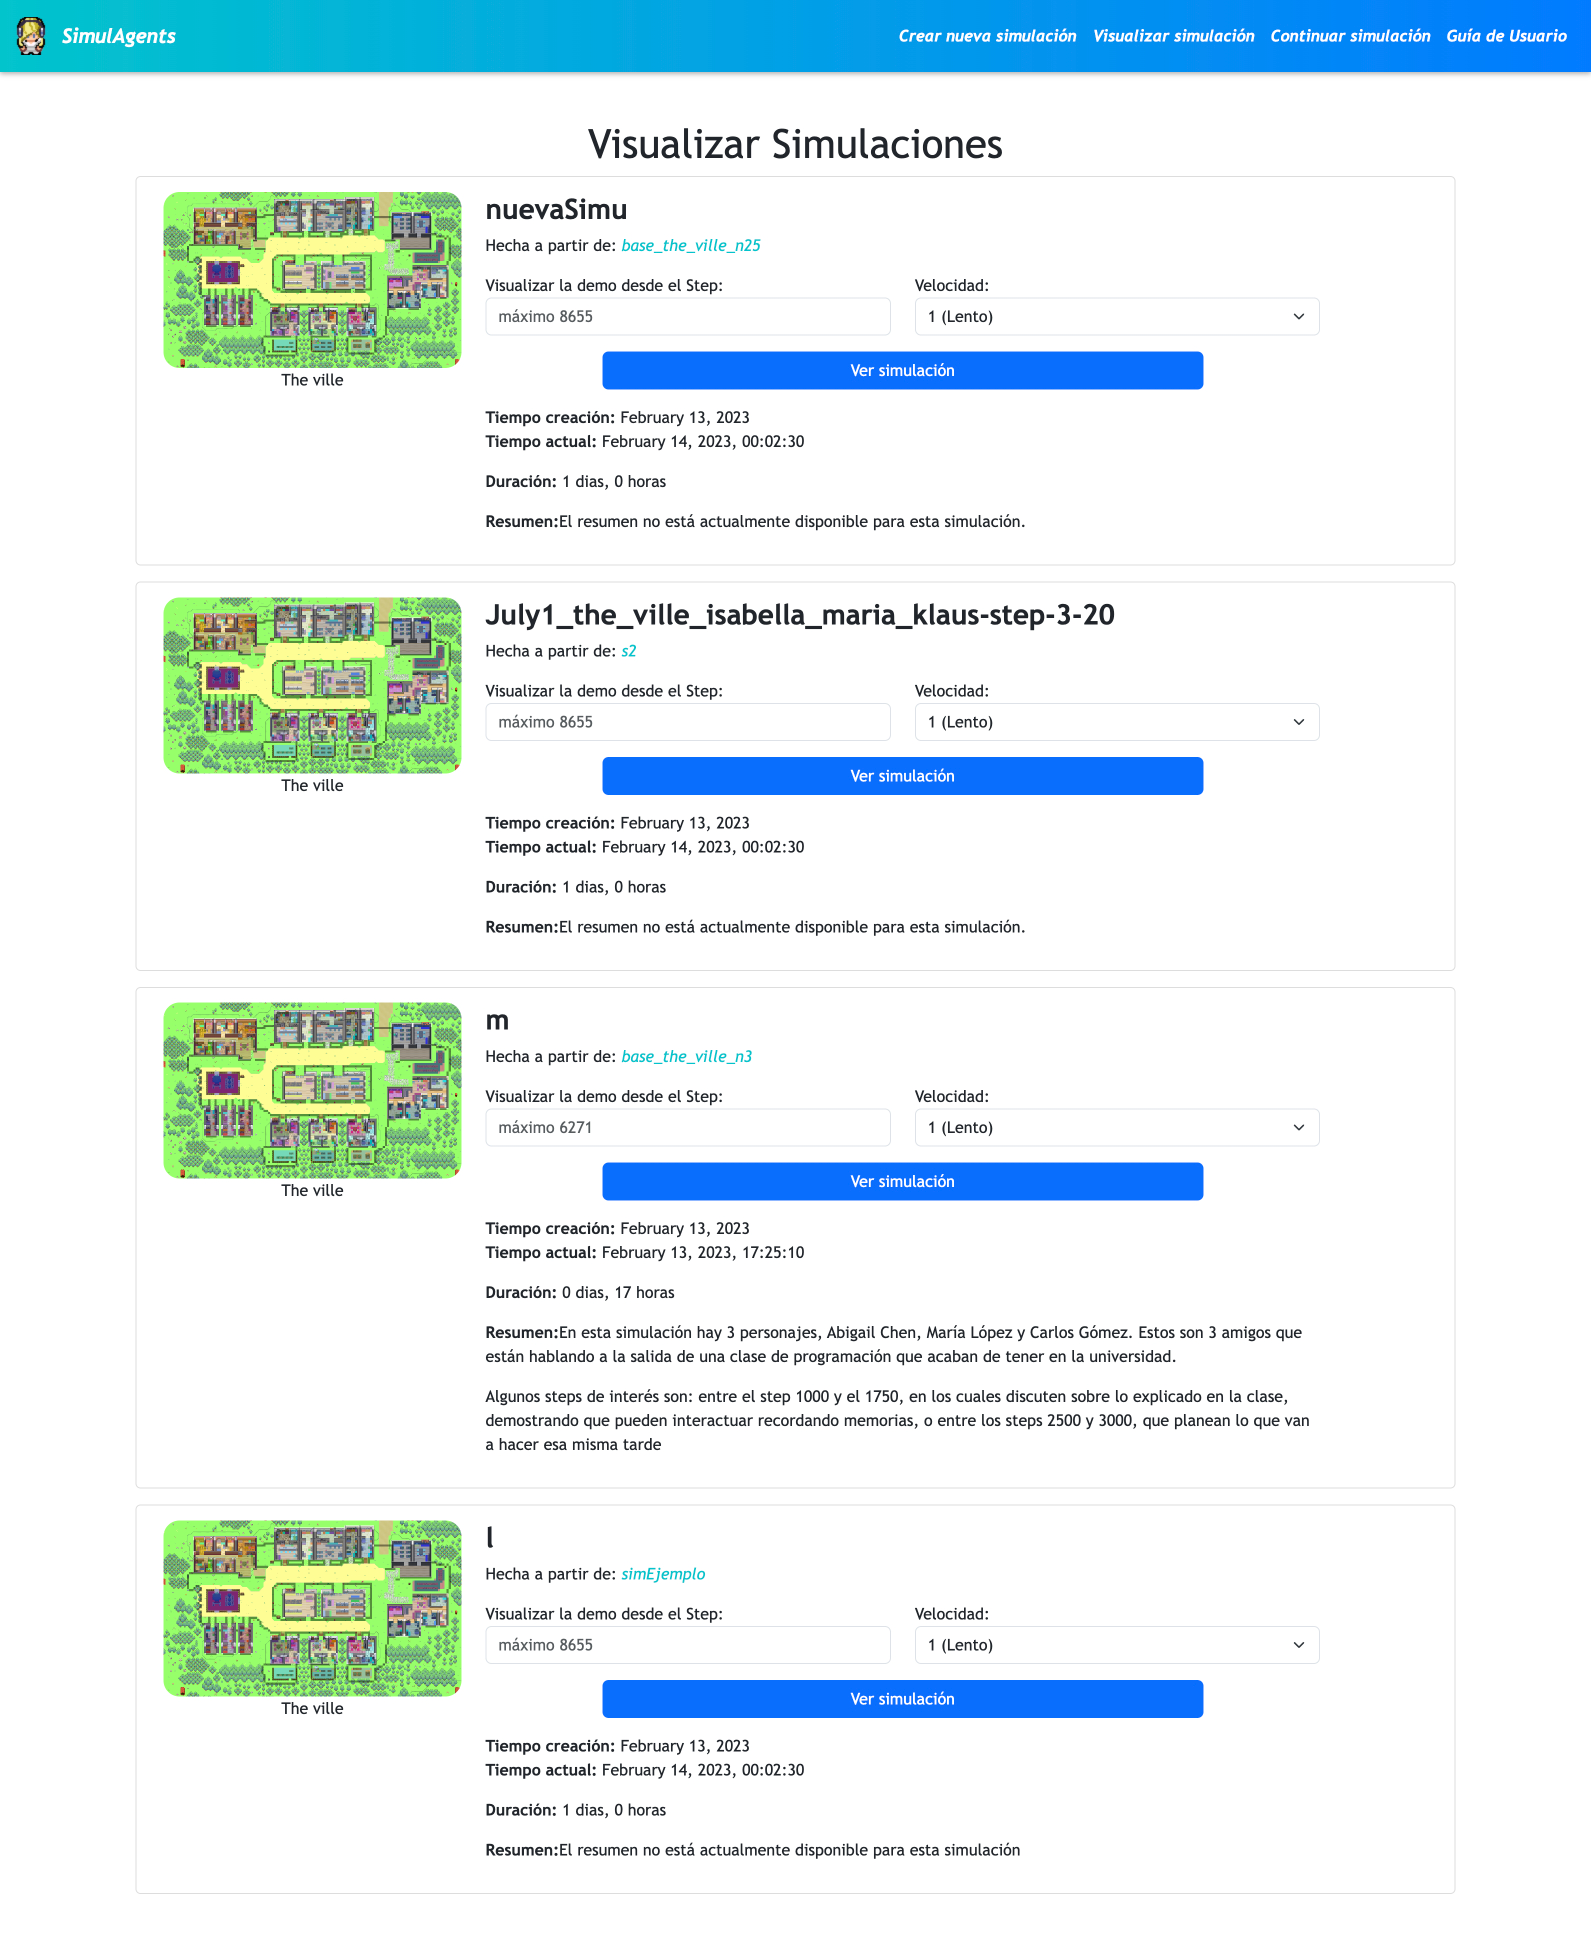
\includegraphics[width = 0.9\textwidth]{Imagenes/Vectorial/vistaVisSimu.png}
	\caption{Vista de visualizar simulaciones en formato escritorio}
	\label{fig:visSimDesktop}
\end{figure}

Esta era una de las interfaces que no existían y tenían mucho sentido en nuestra aplicación. Antes, el usuario debía interactuar directamente con los ficheros y acceder a sus simulaciones mediante la terminal, ahora esto se gestiona automáticamente y se puede acceder mediante un par de clicks, mejorando así la experiencia de usuario, centrando el diseño en el usuario final del sistema.

En este listado de simulaciones finalizadas, se muestra información útil para el usuario como el título de la información, el título de la simulación padre (para que el usuario pueda acceder a ella y continuarla o modificarla), el step desde el que se desea comenzar a visualizar la simulación o la velocidad de reproducción de esta.

Además de esta información, también se genera un resumen automático mediante una llamada al LLM cada vez que se guarda una simulación, el cual se incluye en cada una de las simulaciones, indicando a grandes rasgos lo que ocurre y los steps más interesantes a visualizar.


\subsection{Vista de Continuar simulación}

La vista de continuar simulación es ciertamente similar a la anterior de visualizar simulación, ya que también habrá una lista con simulaciones. Sin embargo, la diferencia crucial entre las simulaciones que se pueden ver y aquellas que se pueden continuar, es que en las segundas, el usuario podrá interactuar directamente con la simulación y alterar el curso de la misma.

De nuevo, es una vista que tenía sentido que existiese, ya que son funcionalidades que estaban muy escondidas y eran difíciles de ejecutar anteriormente, y lo hemos simplificado, permitiendo acceder a ellas mediante una interfaz intuitiva y usable.

En este caso, dado el listado de simulaciones, los usuarios tendrán la opción de continuar la simulación o forkearla, comentaremos las diferencias:

Cuando se continúa una simulación, esta sigue con el mismo nombre y se continúa siempre desde el mismo step. Esta funcionalidad ya estaba disponible, y sirve para continuar una simulación desde el punto en el que el usuario lo había dejado, como indica el nombre.

Sin embargo, al forkear una simulación, se creará una nueva, tomando como base la original. Es por este motivo por el cual, cuando un usuario va a forkear una simulación, se le pide el step desde el que quiere forkearla y se pide que se de un nombre nuevo (ya que será guardada como una nueva simulación en la lista).

 En la figura \ref{fig:contSimDesktop} se puede apreciar el resultado de esta vista, donde se ven una serie de simulaciones que están actualmente disponibles en la aplicación para continuar, así como el número de steps que estas tienen, el nombre de la nueva simulación y más información sobre la simulación en sí (como la duración o los tiempos de la simulación).
 
 \begin{figure}[H]
 	\centering
 	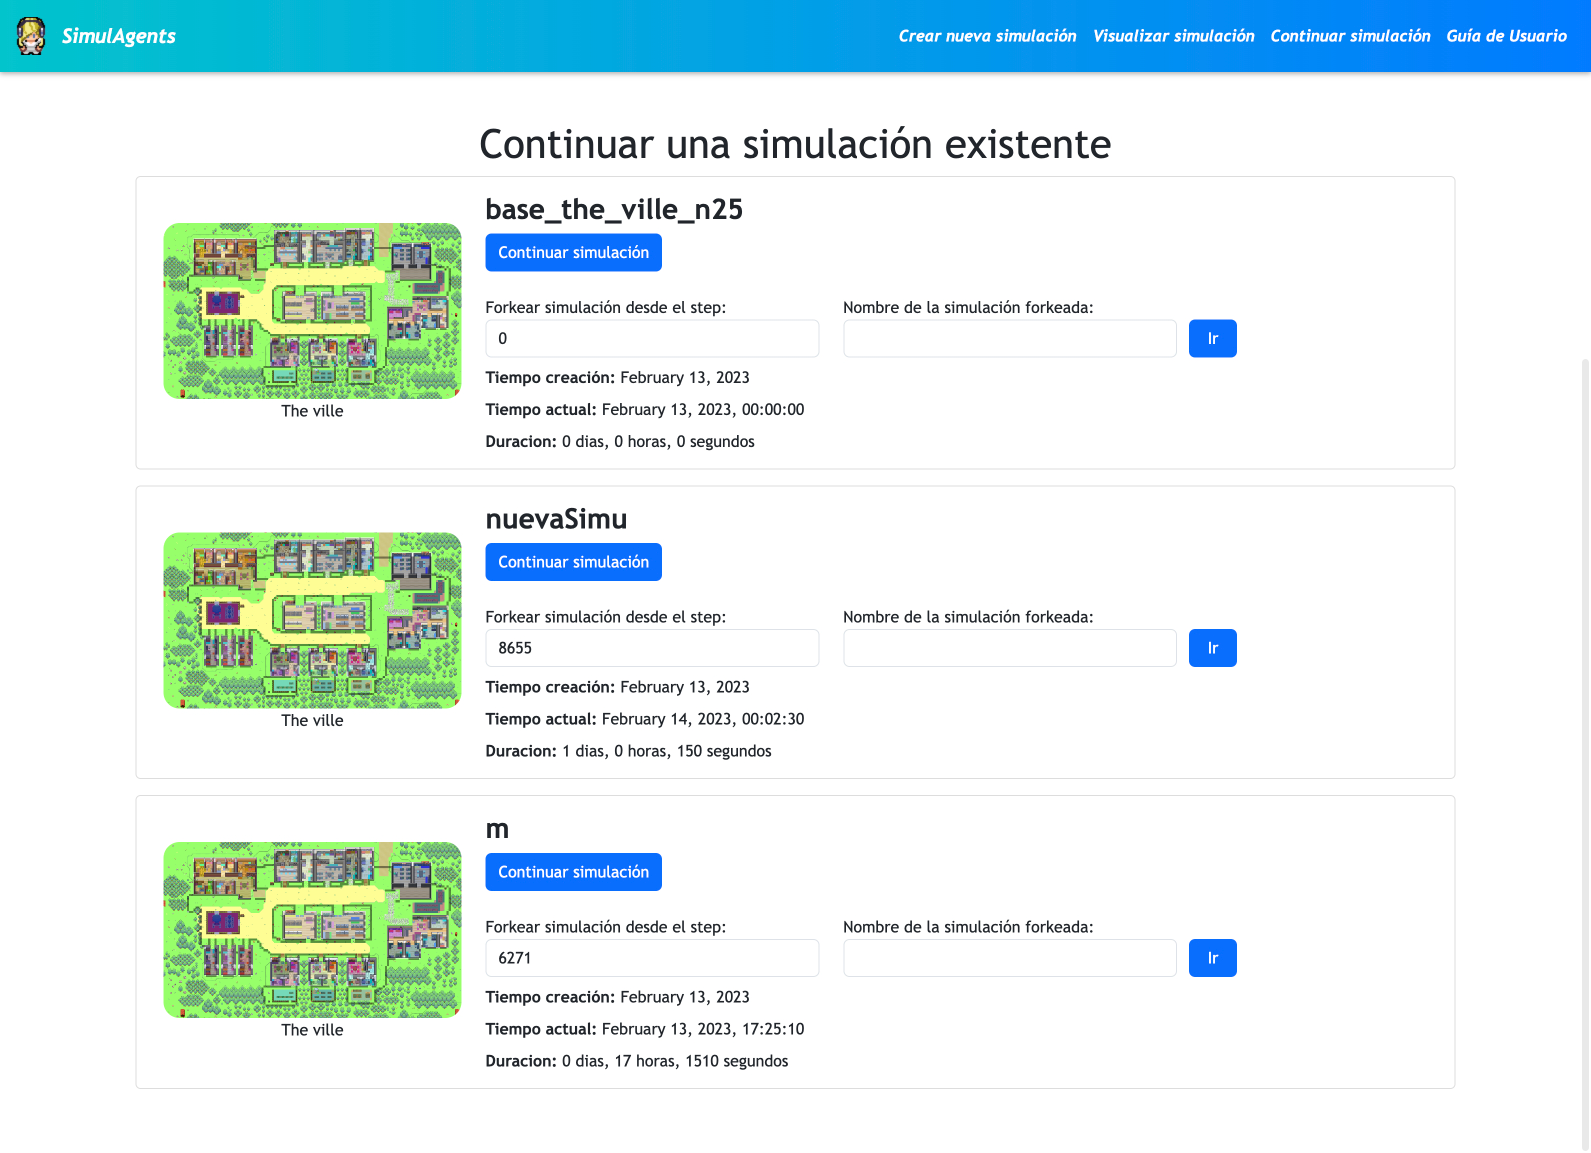
\includegraphics[width = 0.95\textwidth]{Imagenes/Vectorial/vistaContSimu.png}
 	\caption{Vista de continuar simulaciones en formato ecritorio}
 	\label{fig:contSimDesktop}
 \end{figure}

\subsection{Vista de Guía de Usuario}

Además de las vistas creadas para navegar e interactuar con las simulaciones, se ha creado una página que sirve como guía de usuario, que será de utilidad para nuevos usuarios de la aplicación, resolviendo cualquier tipo de dudas acerca de los procesos que se pueden realizar con la aplicación o explicaciones sobre las vistas existentes y cómo usarlas.

Como el uso de esta herramienta lo hemos orientado a perfiles no técnicos (como psicólogos o personas que quieran estudiar las interacciones sociales), se ha añadido esta sección en la que se explican todas las funcionalidades de la aplicación, cómo utilizarlas y algunos trucos o consejos de uso, para maximizar el valor de la aplicación.

En esta guía se hace un repaso extensivo de las vistas existentes en la aplicación, cómo usarlas y para qué sirve cada uno de los botones.

Algunos ejemplos de esta página son los que se muestran en la figura \ref{fig:vistaGuiaUsuario}

 \begin{figure}[H]
	\centering
	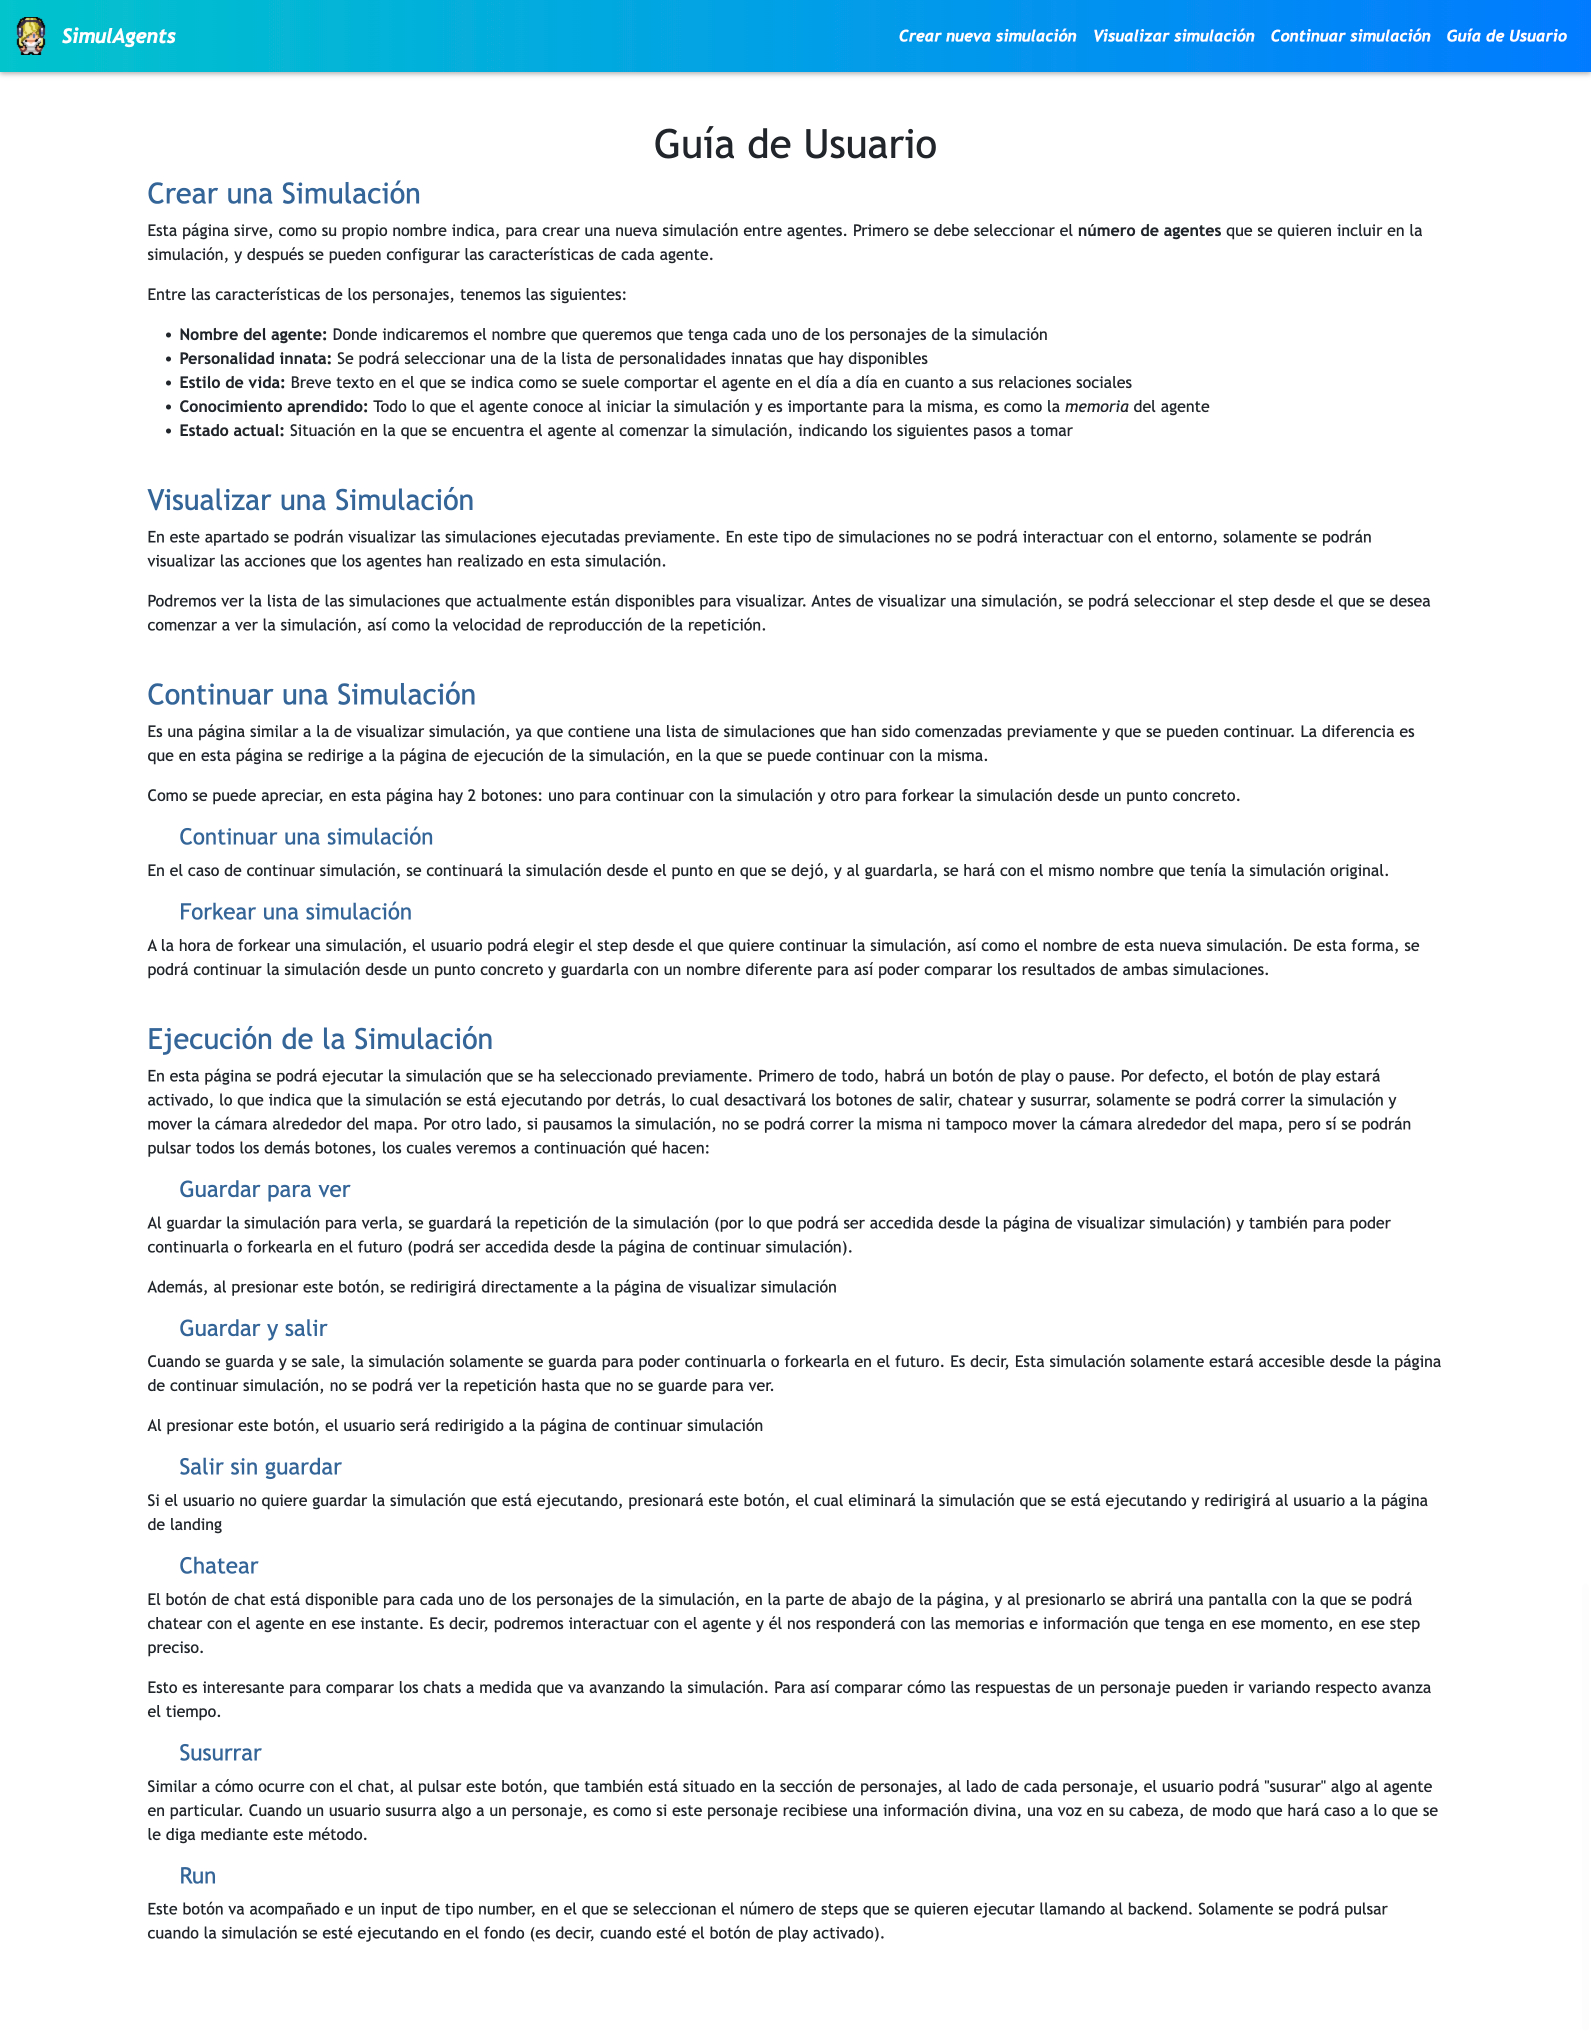
\includegraphics[width = 0.95\textwidth]{Imagenes/Vectorial/vistaGuiaUsuario.png}
	\caption{Vista de la guía de usuario en versión escritorio}
	\label{fig:vistaGuiaUsuario}
\end{figure}

\section{Vistas modificadas}

Además de las vistas creadas desde cero, había algunas que ya estaban creadas (como las de la visualización o ejecución de la simulación, que requerían de un motor de videojuego corriendo). Sin embargo, para añadir ciertas funcionalidades, también se han modificado, las cuales se indican en la presente sección.

\subsection{Vista de landing}

Esta vista se podría considerar como nueva, ya que fue modificada por completo para el propósito de este trabajo.

Originalmente, cuando el usuario arrancaba el servidor, existía una página de landing a la que se le redirigía, donde solamente se indicaba que el servidor se encontraba en funcionamiento con un texto. Como esta página era muy rudimentaria y tan solo contenía una línea de información, se decidió rediseñar la landing completamente, indicando las principales funcionalidades de la aplicación desde una interfaz intuitiva, sencilla y accesible.

Como se puede apreciar en la figura \ref{fig:landing}, hay una breve explicación del trabajo y algunas tarjetas con la información más importante de lo que puede hacer esta aplicación. Se trata de una págia meramente informativa desde la que el usuario puede navegar hacia el resto.

\begin{figure}[H]
	\centering
	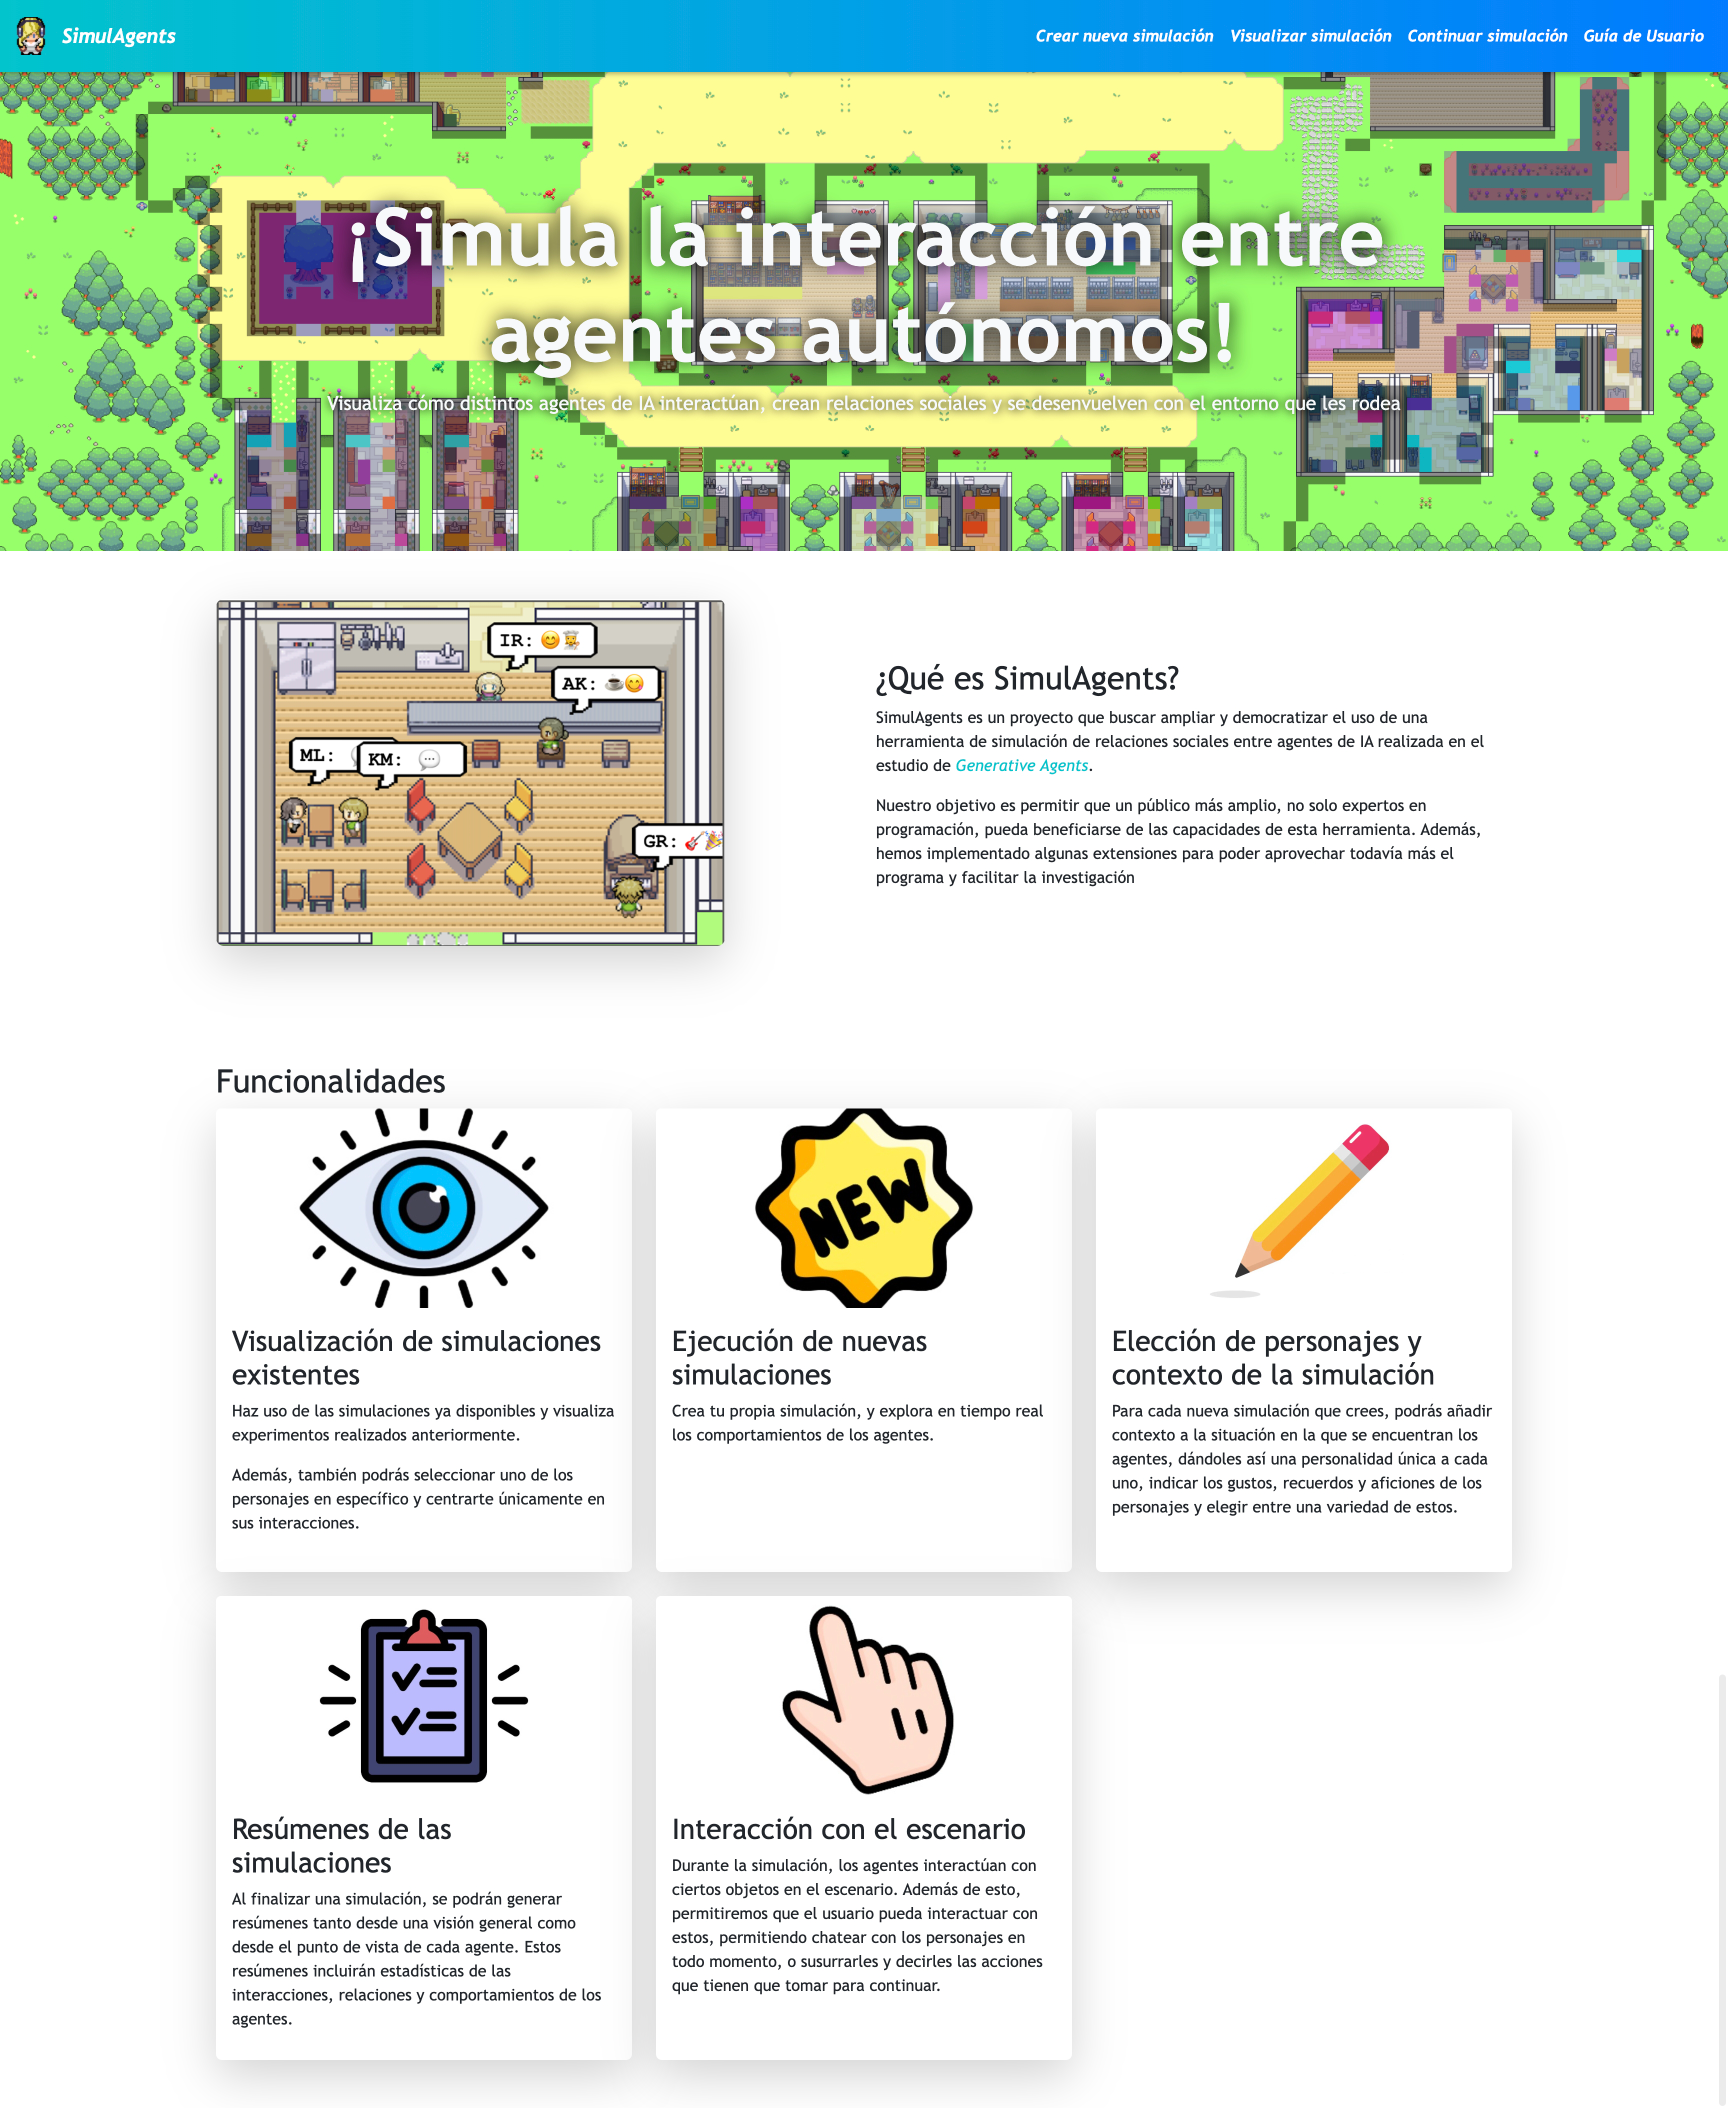
\includegraphics[width = 0.7\textwidth]{Imagenes/Vectorial/landing.png}
	\caption{Vista de landing actualizada}
	\label{fig:landing}
\end{figure}

\subsection{Vista de visualización de una simulación}
\label{sec:vistaSimulacion}

Esta es una de las dos vistas principales que ya existían en la aplicación inicialmente. Esta vista, así como la de ejecución de simulación, existían para que el usuario pudiese ver la simulación y lo que estaba ocurriendo, no estaban pensadas para que el usuario interactuase con ellas y dejarían de tener sentido una vez se pausase la simulación.

Sin embargo, como hemos centralizado todo en un front end común, estas vistas ahora se convierten en algo crucial. Lo más importante de estas vistas es que cogen la información de la simulación y utilizan el motor de juegos Phaser 3.0 para representar el mapa, los personajes y sus movimientos.

El trabajo que hemos realizado en esta vista fue básicamente el de simplificación de la misma (eliminación de botones para ver el estado en profundidad de los personajes) así como la integración de esta vista con el resto de la aplicación (añadido el navbar para navegar en ella).

Un ejemplo de esta vista es el de la figura \ref{fig:verSim}, en la que se visualiza la simulación con nombre 'nuevaSimu', la cual tiene 3 personajes, de los cuales se puede ver su estado y situación en cada momento.

\begin{figure}[H]
	\centering
	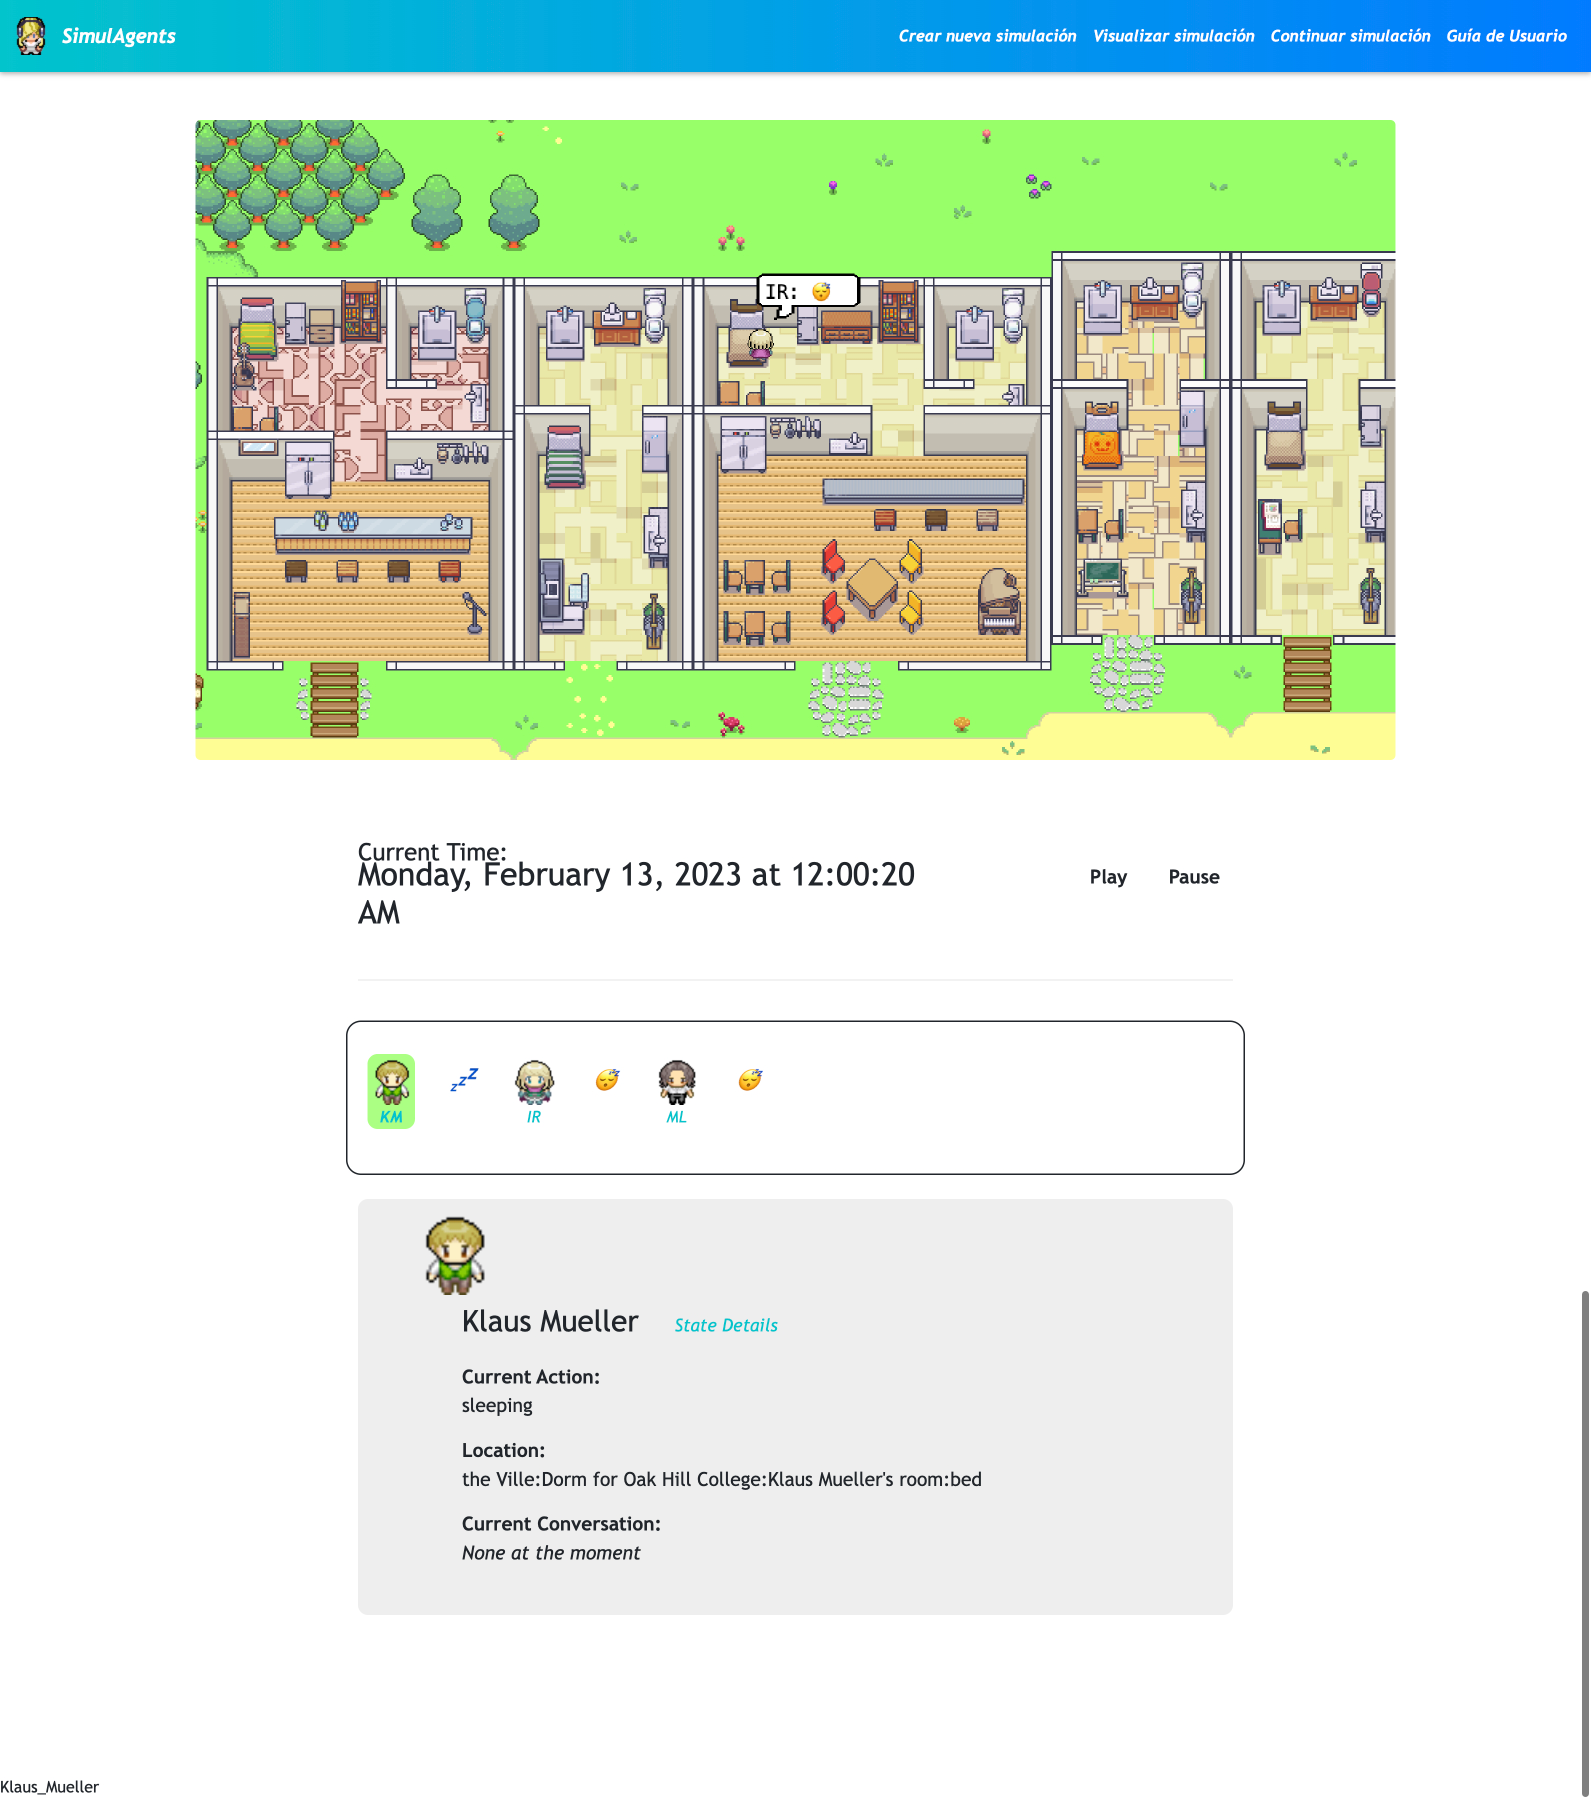
\includegraphics[width = 0.7\textwidth]{Imagenes/Vectorial/vistaVerSim.png}
	\caption{Vista de visualización de una simulación}
	\label{fig:verSim}
\end{figure}


\subsection{Vista de ejecución de simulación}

Como ya se mencionó, esta vista es bastante similar a la comentada en el apartado anterior. Era una vista que ya existía, representando la ejecución de una simulación en tiempo real, con el mismo motor de juegos que se usa a la hora de visualizar una simulación, Phaser 3.0.

No obstante, en esta vista sí que hemos modificado varios elementos y añadido funcionalidades críticas en esta vista, para que el usuario pueda tener una mayor interacción con el sistema en tiempo real. Entre estas modificaciones están los botones de guardar, salir, chat y susurro, de los cuales hablaremos a continuación.

Además, hemos decidido eliminar la barra de navegación de esta página, ya que consideramos que el usuario solo debe salir de esta página si es guardando o saliendo de la presenta simulación (ya sea guardar para verla, para continuarla o eliminarla).

En la figura \ref{fig:vistaEjecSim} podemos ver un ejemplo de esta página en ejecución, en la cual vemos una nueva simulación creada por nosotros, donde hemos añadido dos agentes.

\begin{figure}[H]
	\centering
	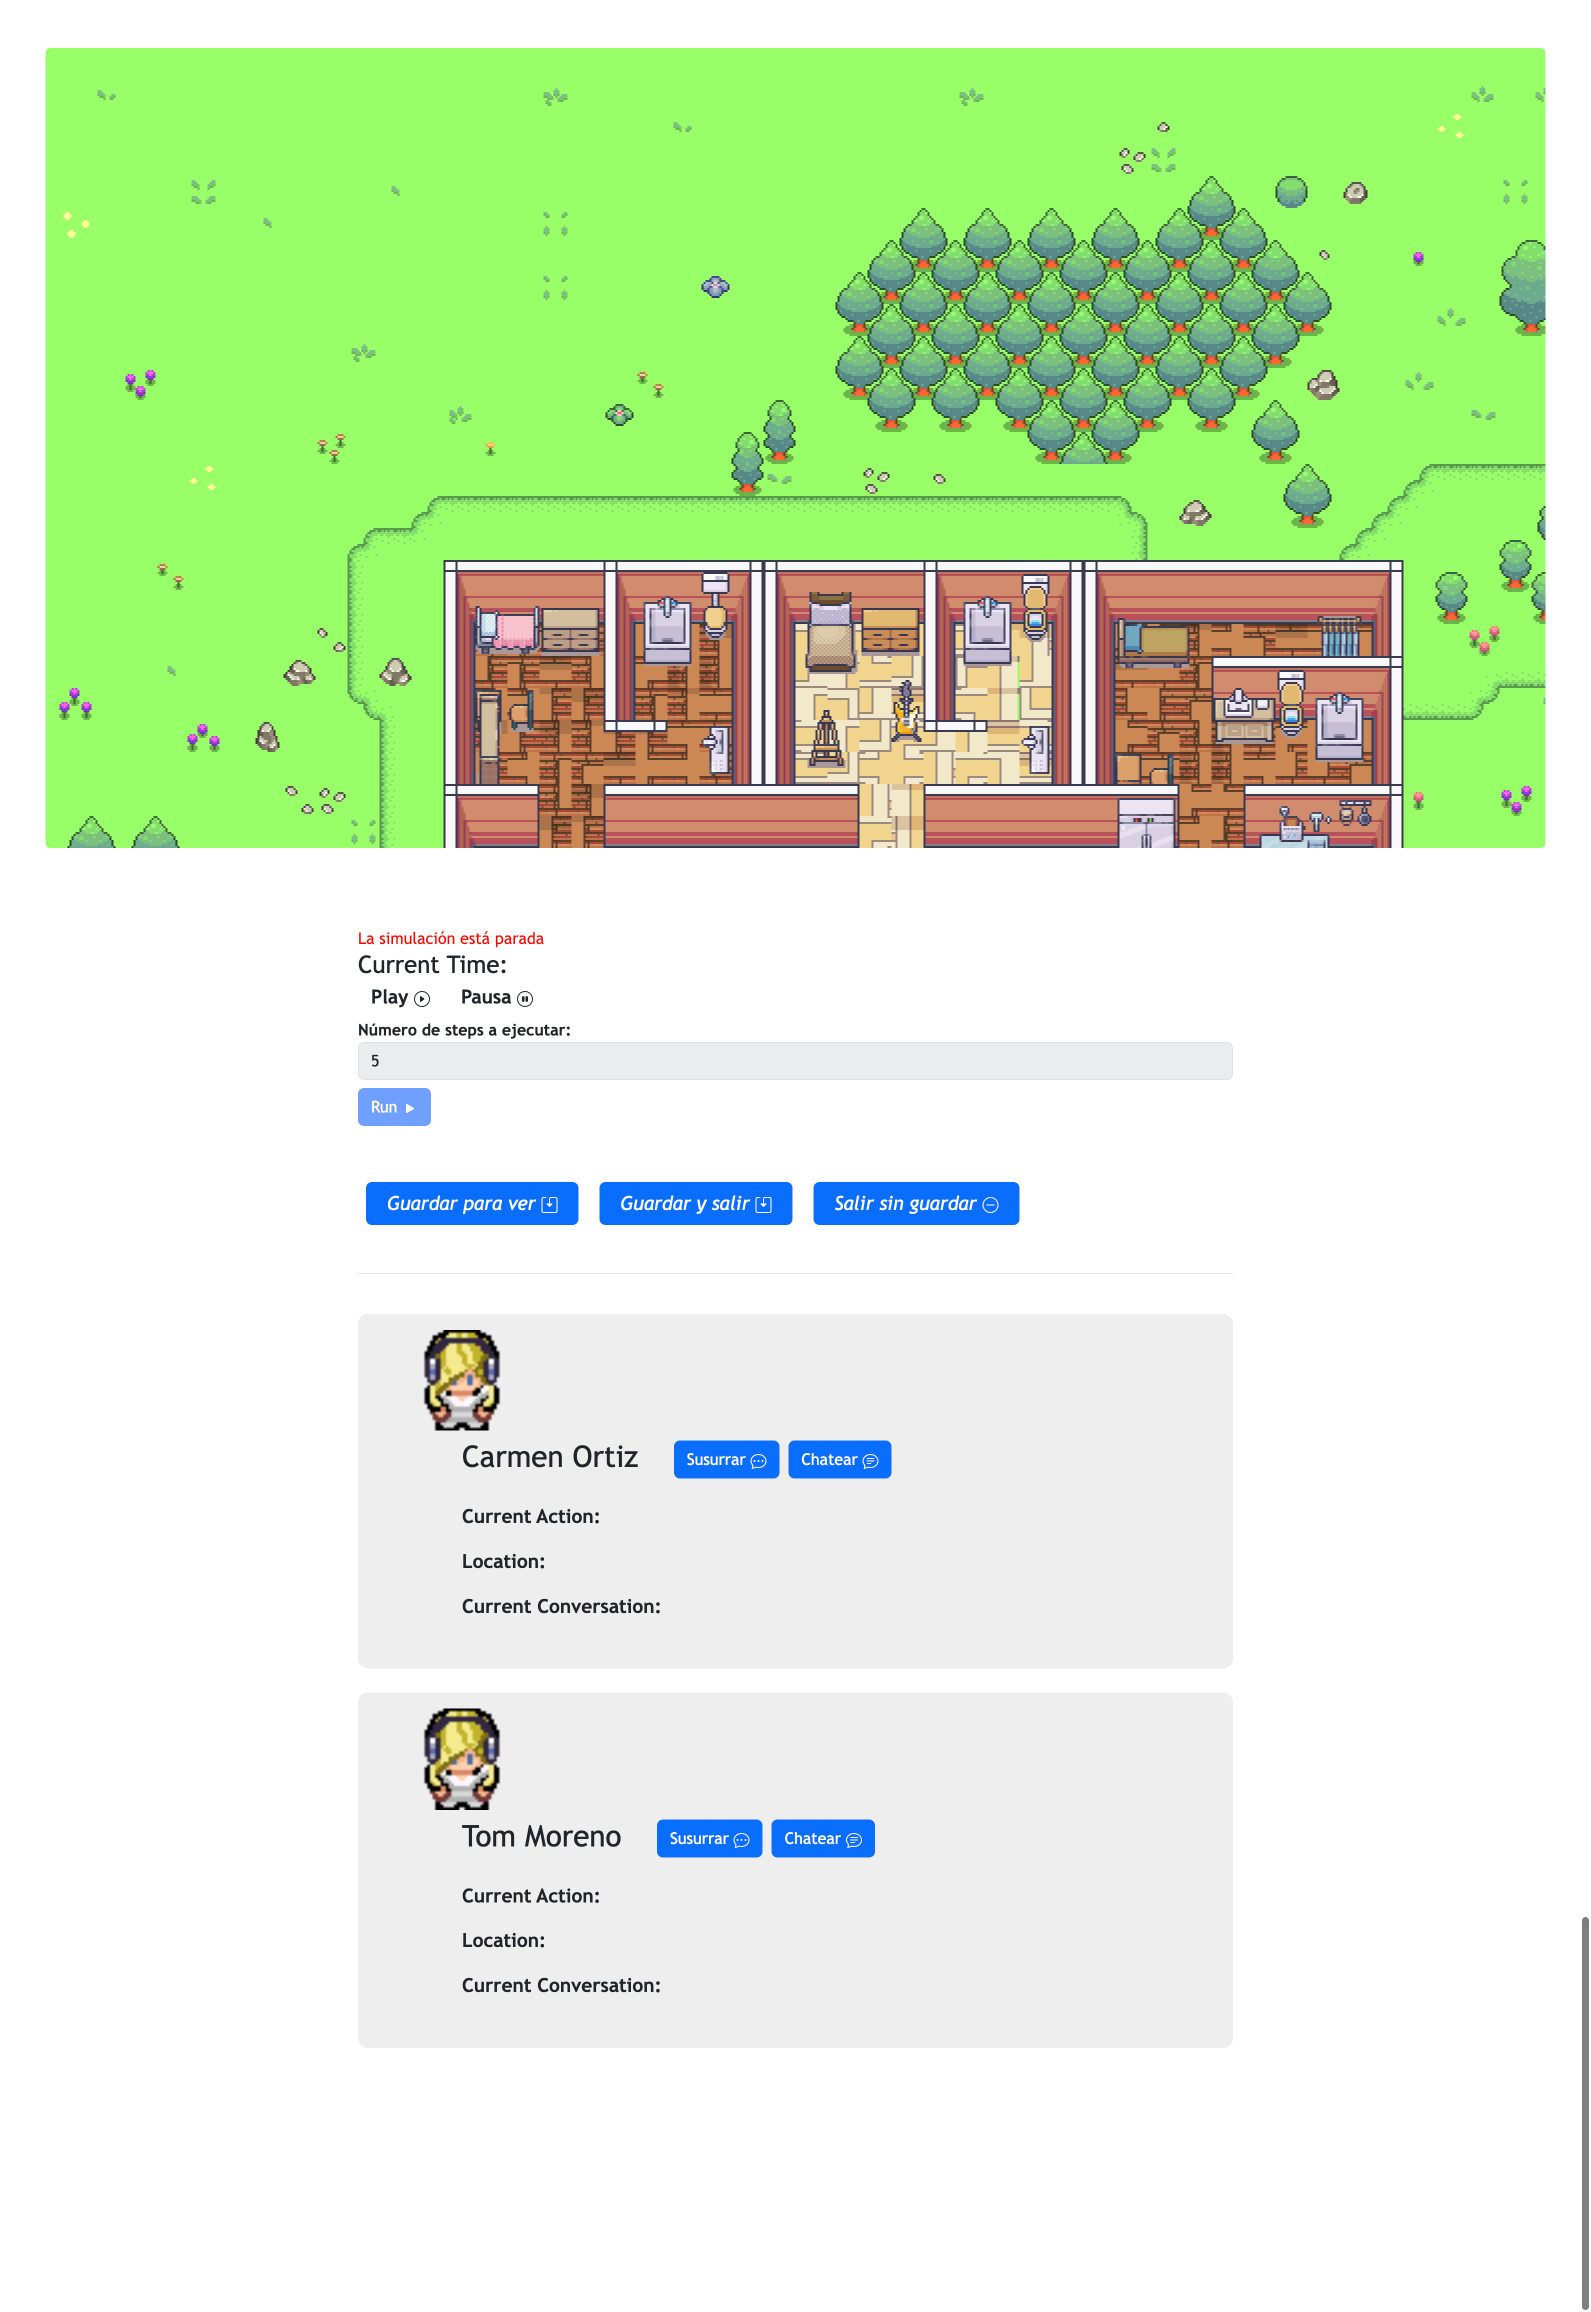
\includegraphics[width = 0.6\textwidth]{Imagenes/Vectorial/ejecucionSimu.png}
	\caption{Vista de ejecución de una simulación}
	\label{fig:vistaEjecSim}
\end{figure}

Las modificaciones que hemos realizado en esta página de ejecución de la simulación se explican a continuación en detalle:

\subsubsection{Botón de 'play'}

Para empezar, se distinguen dos estados de la simulación. Cuando la simulación está corriendo en segundo plano, se podrá hacer run de la simulación, pero no se podrá interactuar directamente con los personajes ni guardar ni salir de la simulación.

Cuando se carga la página o cuando el usuario pulsa este botón de 'play', la simulación entrará en este modo, en que está corriendo en segundo plano, y se indicará con el texto en color verde de 'La simulación se está ejecutando', como se muestra en la figura \ref{fig:simuEjecutando}.

\begin{figure}[H]
	\centering
	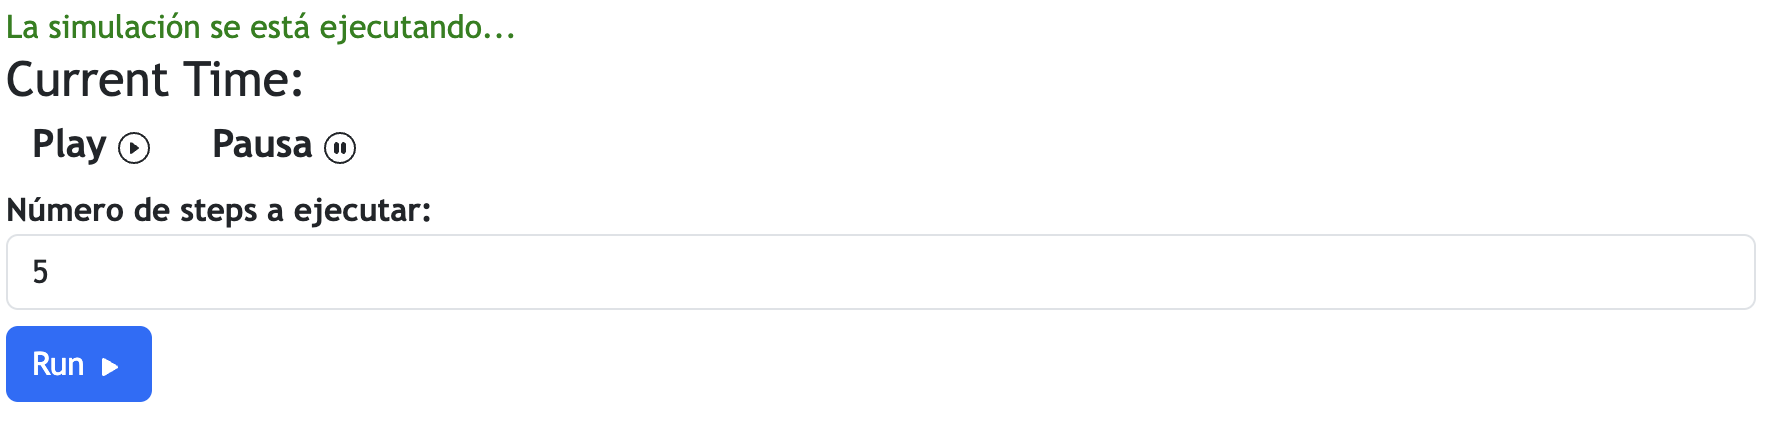
\includegraphics[width = 0.9\textwidth]{Imagenes/Vectorial/simEjecutando.png}
	\caption{Texto indicativo de que la simulación está ejecutando en segundo plano}
	\label{fig:simuEjecutando}
\end{figure}

\subsubsection{Botón de 'pause'}

Por otro lado, existe otro estado en que la simulación está parada, por lo que no se puede ejecutar el botón de 'run', pero sí se podrá guardar, salir, chatear o susurrar a los personajes. Esto se puede ver en el apartado encima de <<Current time>> en la figura \ref{fig:vistaEjecSim}, donde se aprecia en rojo el texto 'La simulación está parada'.

\subsubsection{Botón de 'run'}

Antes, para ejecutar steps de una simulación, era necesario ir a la terminal y ejecutar el comando 'run <número de steps>'. Ahora, hemos implementado un botón de 'run', situado al lado de un input de tipo número, que indicará el número de steps a ejecutar. 

Por ejemplo, si el usuario quiere ejecutar 3 steps, insertará el número en el input y le dará a play, ejecutando así 3 steps y pudiendo verlos en tiempo real en la ventana que contiene la simulación.

\subsubsection{Botones de guardado y salida}

Una vez el usuario considera que ha terminado la simulación, tiene 3 diferentes opciones, que servirán para distintas finalidades, explicadas a continuación:

\begin{itemize}
	
	\item \textbf{Guardar para ver}: Si el usuario desea guardar la simulación y que esté disponible entre aquellas que se pueden visualizar (desde la página de visualizar simulación) deberá darle a este botón. Una vez clicado, se guardará la repetición, la simulación también estará disponible para ser continuada y se redirigirá al usuario a la página de "visualizar simulación", par que pueda ver la nueva repetición.
	
	\item \textbf{Guardar y salir}: Si el usuario quiere guardar la simulación, pero no la repetición, deberá clicar este botón. Al hacerlo, se guardará la simulación para poder continuarla o forkearla, y se redirigirá al usuario a la página de continuar simulación.
	
	\item \textbf{Salir sin guardar}: Al pulsar este botón, el usuario considera que ha terminado la simulación y no desea guardarla. Por lo tanto, se le redirigirá a la página de landing y la simulación se eliminará del sistema. Esta es una funcionalidad nueva ya que no estaba implementada en el sistema original.

\end{itemize}

\subsubsection{Botones de chat y susurro en la vista del personaje}
\label{botonSusurro}

Estos botones están en la sección de personajes. En cada tarjeta de personaje, habrá un botón de chat y otro de susurro. Al clicar en ellos automáticamente se detectará el personaje al cual se quiere susurrar o con el que se quiere chatear en cada caso, y se procederá a ello.

Estas dos funcionalidades son el ejemplo más claro y directo que hay en todo el presente trabajo del uso del procesamiento del lenguaje natural, que se comenta en el capítulo 2 (el Estado de la Cuestión). De todo el sistema, es la única funcionalidad que permite interactuar directamente con el modelo de lenguaje, el cual interpretará el lenguaje natural y lo procesará para devolver una respuesta. En el caso del chat, se comprende la petición del usuario, se interpreta, y se devuelve una respuesta sobre lo que responde el agente. Por otro lado, para el susurro, el usuario interactuará indicando una orden o directriz y el sistema la interpretará para que el usuario la tenga en cuenta y la realice en los siguientes steps de la simulación.

El botón de susurro permite hablar directamente a los pensamientos del personaje e instarle a tomar ciertas decisiones o realizar ciertas acciones. Esta era una funcionalidad preexistente pero la hemos pasado completamente al front. Se puede ver en la figura \ref{fig:cuadroSusurro}, cómo el usuario susurra al personaje de Carmen Ortiz cómo debe reaccionar y actuar a partir de ese momento en la simulación, implementándolo así en su personalidad.

\begin{figure}[H]
	\centering
	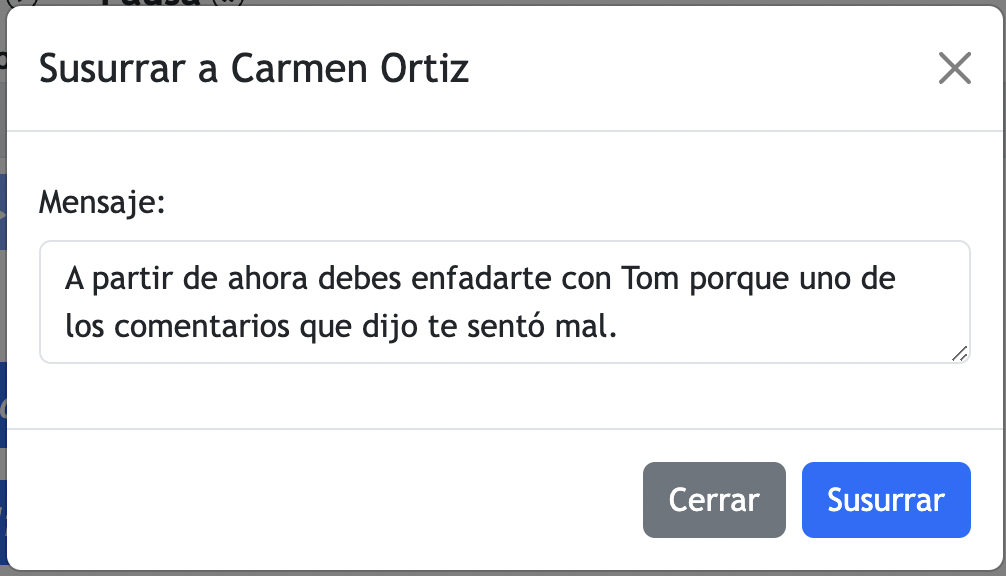
\includegraphics[width = 0.7\textwidth]{Imagenes/Vectorial/cuadroSusurro.png}
	\caption{Modal de susurro}
	\label{fig:cuadroSusurro}
\end{figure}

Por su parte, el botón de chat abrirá una pantalla para chatear directamente con el personaje en tiempo real. Esta funcionalidad es novedosa y servirá para poder entrevisar a los personajes en cada punto de la simulación, viendo así sus cambios de ideas, pensamientos u opiniones a lo largo de la simulación.

En la figura \ref{fig:cuadroChat} se puede apreciar cómo sería la interacción con uno de los personajes de la simulación. Mediante esta interfaz de chat, se interpretaría la entrada del usuario y, mediante procesamiento del lenguaje natural y empleando el LLM, trataríamos de obtener una respuesta coherente a la interacción.

\begin{figure}[H]
	\centering
	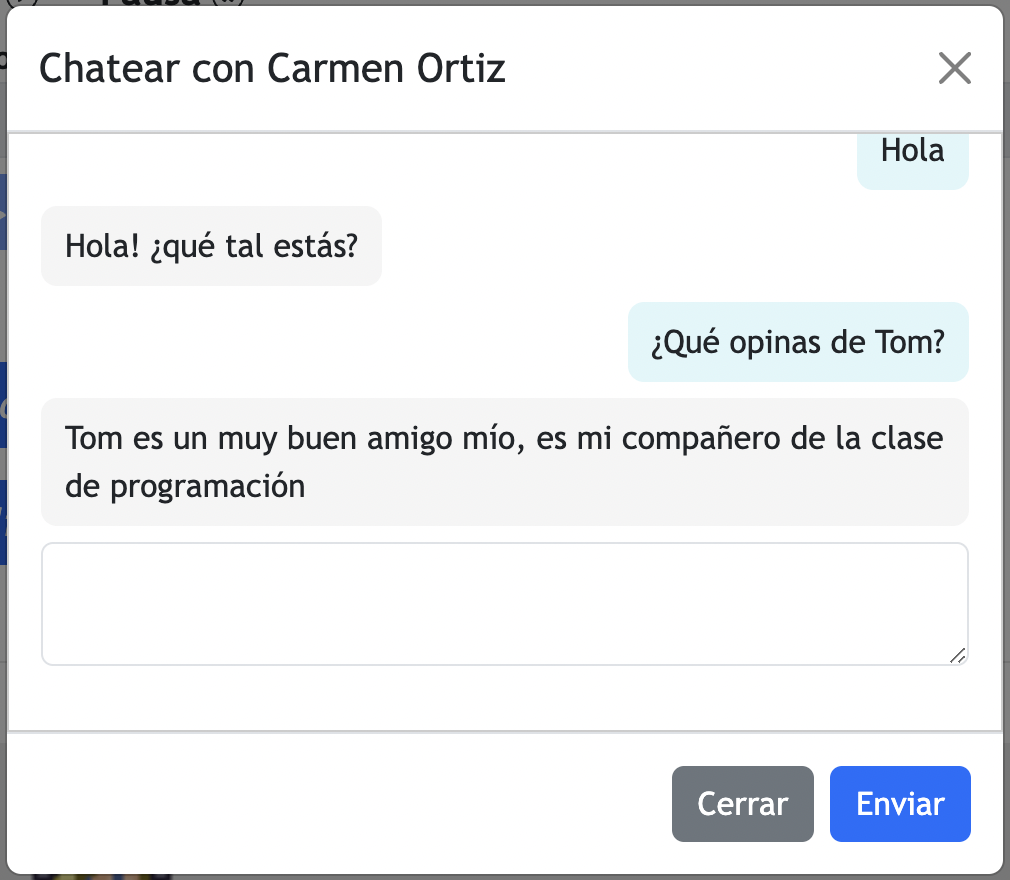
\includegraphics[width = 0.7\textwidth]{Imagenes/Vectorial/cuadroChat.png}
	\caption{Modal de chat con respuestas simuladas}
	\label{fig:cuadroChat}
\end{figure}



